\title{Microkernel Architecture}
\author{Richard Thomas}
\date{\week{3}}

\maketitle

\section{Introduction}

The microkernel architecture aims to deliver sophisticated software systems while maintaining the quality attributes of simplicity and extensibility.
This is achieved by implementing a simple core system that is extended by plug-ins that deliver additional system behaviour.
Microkernel is also known as a ``plug-in'' architecture.

Many common applications use the microkernel architecture.
Web browsers, many IDEs (notably Eclipse), Jenkins, and other tools all use this architecture.
They deliver their core functionality and provide a plug-in interface that allows it to be extended.
\link{Eclipse}{https://www.eclipse.org/downloads/packages/} is famous as a simple text editor that
can be extended to be a sophisticated software development tool through its plug-in interface.

\vspace{2mm}
\begin{definition}[Microkernel Architecture]
    A core system providing interfaces that allow plug-ins to extend its functionality.
\end{definition}

\begin{figure}[h!]
    \centering
    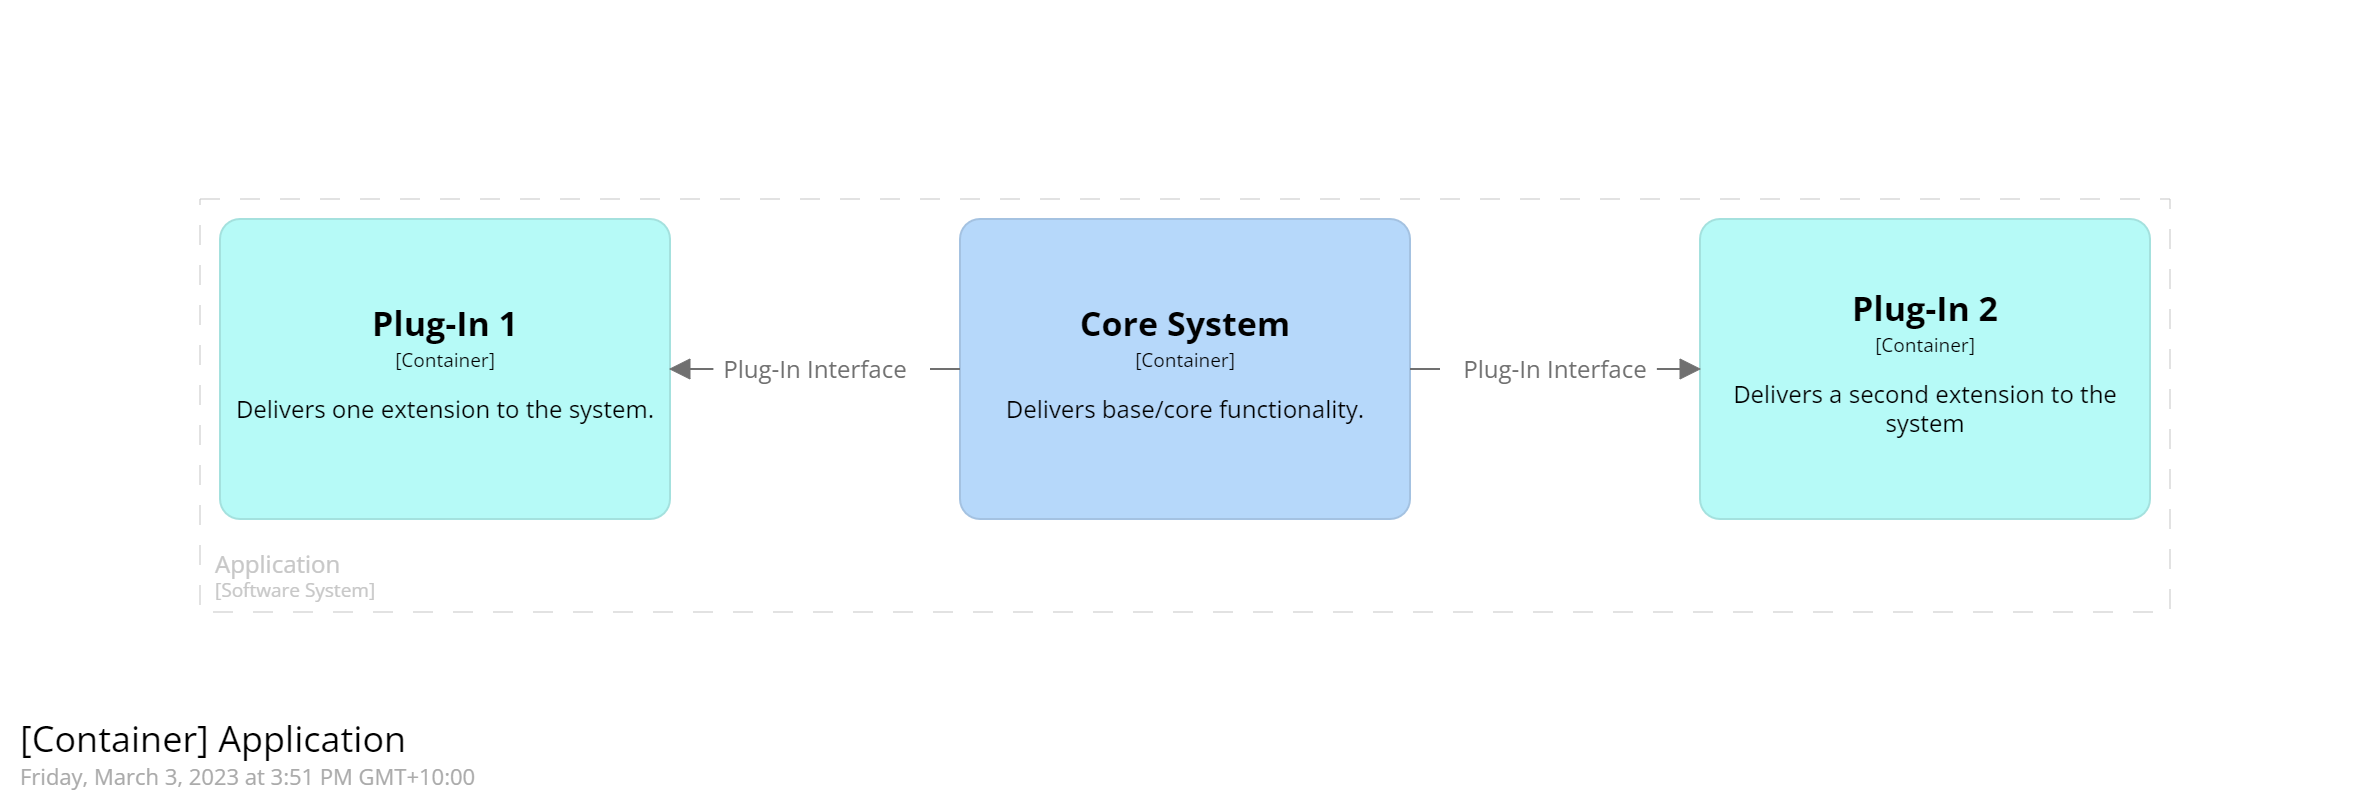
\includegraphics[trim=38 120 22 110,clip,width=0.85\textwidth]{diagrams/generic-microkernel.png}
    \caption{Microkernel architecture -- generic structure.}
    \label{fig:microkernel}
\end{figure}

For example, a web browser provides the core behaviour of rendering web pages.
Plug-ins extend the browser with specialised behaviour, such as a PDF viewer or dark mode reader.


\section{Terminology}

The microkernel architecture consists of four elements.
The \emph{core system}, \emph{plug-ins} and \emph{plug-in interface} shown in figure \ref{fig:microkernel}, plus a \emph{registry}.

\begin{description}
    \item[Core system] implements the system's base functionality.
    \item[Plug-ins] extend the system by providing independent, specialised behaviour.
    \item[Plug-in interface] describes how the core system and plug-ins interact.
    \item[Registry] tracks which plug-ins are available to the core system and how to access them.
\end{description}

The core system implements the minimal functionality that provides the base, or framework, of the system.
This may be the core functionality of the system, like the Eclipse text editor or a web browser's page rendering engine.
Alternatively, the core system may implement a general processing path, like a payroll system's payment process.

The payment process may be simply, identify an employee, calculate their fortnightly pay, and send payment to their bank account.
Calculating pay can be a very complex process\footnote{See the Queensland Health payroll disaster
\url{https://www.henricodolfing.com/2019/12/project-failure-case-study-queensland-health.html}}.
There are different pay rates, bonuses, incentives, salaried staff, staff paid commission, staff paid hourly rates,
overtime rates, penalty rates, deductions, taxes, and many other pay related calculations to consider for each individual.

Plug-ins are independent components that extend the behaviour of the core system.
The simple approach is that the system is delivered as a monolith, including the core system and the plug-in.
In this case the core system uses the plug-in via a method invocation.

In the payroll example, plug-ins can remove the complexity of different pay adjustment calculations from the core system, by moving each calculation to a separate component.
This also improves extensibility, maintainability and testability of the system.
New calculations can be added to the system by implementing a new plug-in.
As each plug-in is independent of the others, it is easier to implement a new calculation, or changing an existing one, than trying to do so in a large monolith.
New plug-ins can be tested independently and then integrated into the system for system testing.

There is usually a single standard interface between the core system and the plug-ins for a domain.
The interface defines the methods that the core system can invoke, data passed to the plug-in, and data returned from the plug-in.
The plug-in component implements the interface and delegates responsibilities within the component to deliver its behaviour.

Figure \ref{fig:interface} is an example of a possible interface for the pay adjusment calculation plug-ins.
Each pay adjustment plug-in returns a \texttt{MonetaryAmount} indicating the amount by which the employee's base pay is to be adjusted in the pay period.
The amount may be positive or negative.
The \texttt{employee}, \texttt{periodDetails}, \texttt{employeeConditions} and \texttt{basePay} objects are passed as parameters to the plug-in.
The plug-in can extract the data it needs from these objects to perform its calculation.
The \texttt{periodDetails} object provides data about the work performed by the employee during the pay period (e.g. time worked, overtime, higher duties adjustments, ...).
The \texttt{employeeConditions} set provides data about each of the employee's pay conditions (e.g. before tax deductions, union membership, ...).

\begin{figure}[ht]{\textwidth}
\centering
\begin{shaded}
\begin{lstlisting}[style=java]
public interface PayAdjustmentPlugin {
    public MonetaryAmount adjustPay(Employee employee,
                                    WorkDetail periodDetails,
                                    Set<Condition> employeeConditions,
                                    MonetaryAmount basePay);
}
\end{lstlisting}
\end{shaded}
\caption{Plug-in interface example for payroll system.}
\label{fig:interface}
\end{figure}

The registery records which plug-ins are available to the core system and how they are accessed.
For the simple case of plug-ins being used by method invocation,
the registry just needs to record the name of the plug-in and a reference to the object that implements the plug-in's interface.
For the payroll example, this could be a simple map data structure.
The core system could lookup a plug-in by its name and then apply it by invoking the \texttt{adjustPay} method on the plug-in object.

\section{Microkernel Principles}
While the concept of a microkernel architecture is straightforward,
there are some principles which should be maintained to produce a maintainable and extendable architecture.

\begin{definition}[Independent Plug-in Principle]
    Plug-ins should be independent, with no dependencies on other plug-ins.
    The only dependency on the core system is through the plug-in interface.
\end{definition}

\todo{Provide commentary about the Independent Plug-in Principle.}

\begin{definition}[Standard Interface Principle]
    ...
\end{definition}

\todo{Provide commentary about the Standard Interface Principle.}



\section{Extensions}

While the core system is often a monolith and it, along with all its plug-ins, is often deployed as a single monolith
(e.g. a web browser), that is not the only approach to using the microkernel architecture.

\todo{Describe variations on the microkernel architecture and distribution options.
This includes using the Adapter design pattern for components that don't implement the standard interface.}


\section{Conclusion}

%A pipeline architecture is a good choice for data processing when interactivity is not a concern.
%Conceptually pipelines are very simple.
%Following the principles of a pipeline architecture will deliver a modular system which supports high reuse.
